\newpage
\section{Cylindre et cône} 
\defn[Cylindre de révolution]{Un \textbf{cylindre de révolution} est une surface engendrée par la révolution autour d'un axe, d'une droite $d$ parallèle à cet axe. Les droites générant le cylindre sont appelées \textbf{génératrices}.}

%% TIKZ : Cylindre
\vspace{0.5cm}
\begin{figure}[H]
\begin{tikzpicture}[scale=1.2]


\comments{
% Axes
\coordinate (xStart) at (1.5,-4,0); % visible starts at intersection with d
\coordinate (xEnd) at (3,-4,0);     % exterior end
\draw[->] (xStart) -- (xEnd) node[anchor=south]{$x$}; % solid visible part
\draw[dashed] (0,-4,0) -- (xStart);

\coordinate (zStart) at (0,0,0); % visible starts at intersection with d
\coordinate (zEnd) at (0,1,0);     % exterior end
\draw[->] (zStart) -- (zEnd) node[anchor=north west]{$z$}; % solid visible part
\draw[dashed] (0,-4,0) -- (zStart);



\coordinate (yStart) at (0,-4,-4); % visible starts at intersection with d
\coordinate (yEnd) at (0,-4,-5);     % exterior end
\draw[->] (yStart) -- (yEnd) node[anchor=south]{$y$}; % solid visible part
\draw[dashed] (0,-4,0) -- (yStart);
}
\coordinate (zStart) at (0,0,0); % visible starts at intersection with d
\coordinate (zEnd) at (0,1,0);     % exterior end
\draw[dashed] (0,-5,0) -- (zEnd);

% Cylinder parameters
\def\radius{1.5}   % radius of the cylinder
\def\height{4}     % cylinder height

% Draw side lines
\draw[thick] (\radius,0) -- (\radius,-\height);
\draw[thick] (-\radius,0) -- (-\radius,-\height);

% Draw top ellipse (centered at (0,0))
% Front half (solid)
\draw[dashed] (0,0) ++(\radius,0) arc [start angle=0,end angle=180,x radius=\radius,y radius=0.5];
% Back half (dashed)
\draw[thick] (0,0) ++(-\radius,0) arc [start angle=180,end angle=360,x radius=\radius,y radius=0.5];

\fill(0,0) circle (1.5pt);

% Draw bottom ellipse (centered at (0,-\height))
% Front half (solid)
\draw[dashed] (0,-\height) ++(\radius,0) arc [start angle=0,end angle=180,x radius=\radius,y radius=0.5];
% Back half (dashed)
\draw[thick] (0,-\height) ++(-\radius,0) arc [start angle=180,end angle=360,x radius=\radius,y radius=0.5];
\fill(0,-\height) circle (1.5pt);

% Infinite generating lines d
\coordinate (TopRight) at (\radius,0);
\coordinate (BaseRight) at (\radius,-\height);
\coordinate (TopLeft) at (-\radius,0);
\coordinate (BaseLeft) at (-\radius,-\height);

\draw[dashed] ($ (BaseRight)!1.2!(TopRight) $) -- ($ (BaseRight)!-0.2!(TopRight) $);
\draw[dashed] ($ (BaseLeft)!1.2!(TopLeft) $) -- ($ (BaseLeft)!-0.2!(TopLeft) $);

% Label the generating line
\path (BaseRight) -- (TopRight) coordinate[pos=-0.2] (midLine);
\node[right] at (midLine) {$d$};


\end{tikzpicture}
\hfill
%% TIKZ : Cone
    \begin{tikzpicture}[scale=1.2]
\comments{
% Axes
\coordinate (xStart) at (1.5,-4,0); % visible starts at intersection with d
\coordinate (xEnd) at (3,-4,0);     % exterior end
\draw[->] (xStart) -- (xEnd) node[anchor=south]{$x$}; % solid visible part
\draw[dashed] (0,-4,0) -- (xStart);

\coordinate (zStart) at (0,0,0); % visible starts at intersection with d
\coordinate (zEnd) at (0,1,0);     % exterior end
\draw[->] (zStart) -- (zEnd) node[anchor=north west]{$z$}; % solid visible part
\draw[dashed] (0,-4,0) -- (zStart);

\coordinate (yStart) at (0,-4,-2.2); % visible starts at intersection with d
\coordinate (yEnd) at (0,-4,-4);     % exterior end
\draw[->] (yStart) -- (yEnd) node[anchor=south]{$y$}; % solid visible part
\draw[dashed] (0,-4,0) -- (yStart);
}

\coordinate (zStart) at (0,0,0); % visible starts at intersection with d
\coordinate (zEnd) at (0,1,0);     % exterior end
\draw[dashed] (0,-5,0) -- (zEnd);

% Cone parameters
\def\radius{1.5}    % maximum radius
\def\height{2}      % half of cone height
\def\sommet{-2}

\coordinate (Apex) at (0,\sommet,0);
\coordinate (BaseRight) at (\radius,-\height+\sommet,0);
\coordinate (BaseLeft) at (-\radius,-\height+\sommet,0);

\fill(Apex) circle (2pt) node[anchor=east]{$V$};
% Bottom cone (positive z)
\draw[thick] (-\radius,-\height+\sommet) -- (0,\sommet);
\draw[thick] (\radius,-\height+\sommet) -- (0,\sommet);

% Draw base ellipse (split front/back)
% Front half (solid)
\draw[dashed] (0,-\height+\sommet,0) ++(\radius,0) 
    arc[start angle=0,end angle=180,x radius=\radius,y radius=0.4];
% Back half (dashed)
\draw[thick] (0,-\height+\sommet,0) ++(-\radius,0) 
    arc[start angle=180,end angle=360,x radius=\radius,y radius=0.4];

\fill(0,-\height+\sommet,0) circle (1.5pt);
% Top cone (negative z)
\draw[thick] (-\radius,\height+\sommet) -- (0,\sommet);
\draw[thick] (\radius,\height+\sommet) -- (0,\sommet);
%\draw[dashed] (0,\height+\sommet) ellipse (\radius cm and 0.4 cm);
% Front half (solid)
\draw[dashed] (0,\height+\sommet,0) ++(\radius,0) 
    arc[start angle=0,end angle=180,x radius=\radius,y radius=0.4];
% Back half (dashed)
\draw[thick] (0,\height+\sommet,0) ++(-\radius,0) 
    arc[start angle=180,end angle=360,x radius=\radius,y radius=0.4];
\fill(0,\height+\sommet,0) circle (1.5pt);
% Draw the infinite generating line d with dashed extension
\draw[dashed] 
  ($ (BaseRight)!2.2!(Apex) $) -- 
  ($ (BaseRight)!-0.2!(Apex) $);
\draw[dashed] 
  ($ (BaseLeft)!2.2!(Apex) $) -- 
  ($ (BaseLeft)!-0.2!(Apex) $);

% Optional: center line along z-axis
\draw[dashed] (0,0) -- (0,\height+\sommet);
\draw[dashed] (0,0) -- (0,-\height+\sommet);


% Label the generating line d
% Place the label midway along the right side
\path (BaseRight) -- (Apex) coordinate[pos=-0.2] (midLine);
\node[right] at (midLine) {$d$};

\end{tikzpicture}

\end{figure}

\vspace{0.5cm}


\defn[Cône de révolution]{Un \textbf{cône de révolution} est une surface engendrée par la révolution autour d'un axe, d'une droite $d$ sécante à cet axe. L'intersection entre la droite et l'axe de révolution est le sommet $V$ du cône.Les droites générant le cône sont appelées \textbf{génératrices}.}
\\~
\vspace{2cm}
\rap{Tangente à un cercle ? Tangente à une sphère ?}

\newpage
\lemma{Soit une sphère $\mathcal{S}$ et un point $V$ fixé à l'extérieur de $\mathcal{S}$. Tous les segments reliant $V$ à un point $M$ de la sphère, de sorte que la droite $VM$ soit tangente à la sphère $\mathcal{S}$, ont la même longueur.} \label{lemme_c_s}


\begin{minipage}{0.45\textwidth} % left side: figure
\begin{figure}[H]
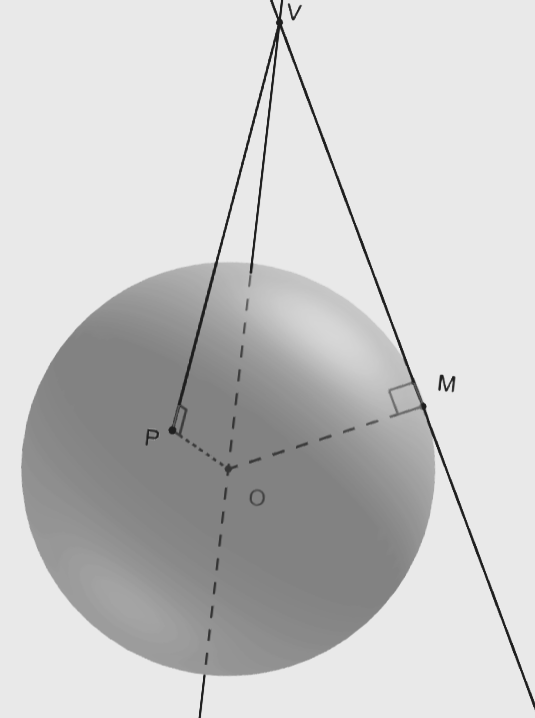
\includegraphics[width = 7cm]{./images/3d/lemme_1_nb.PNG}
\end{figure}
\end{minipage}
\hfill
\begin{minipage}{0.5\textwidth} % right side: text
\begin{proof}
    \hspace{0.6\textwidth}

     Soit $O$, le centre de la sphère $\mathcal{S}$ de rayon $R$, et $V$ un point extérieur à $\mathcal{S}$.\\
La distance $\overline{OV}= L$ est donnée et fixe.\\
Considérons un point $M\in\mathcal{S}$ tel que la droite $VM$ soit tangente à $\mathcal{S}$.\\
Par définition de la tangente, le segment $[OM]$ est perpendiculaire à $[VM]$.\\
Donc, le triangle $\triangle VMO$ est rectangle en $M$.\\
Par Pythagore, nous avons $\overline{OV}^2 = \overline{VM}^2+ \overline{OM}^2$.\\
Comme $\overline{OM} = R$ et $\overline{OV}=L$, alors\\ $\overline{VM} = \sqrt{L^2 - R^2}$ et est la même pour tout point $M$ de la sphère tel que $VM$ soit tangent à la sphère.
\end{proof}

\end{minipage}

\vspace{0.5 cm}
\lemma{Le lieu des points  $M$ de tangence d'une sphère inscrite à un cône est un cercle.}\label{lemme_cercle}

\begin{minipage}{0.4\textwidth} % left side: figure
\begin{figure}[H]
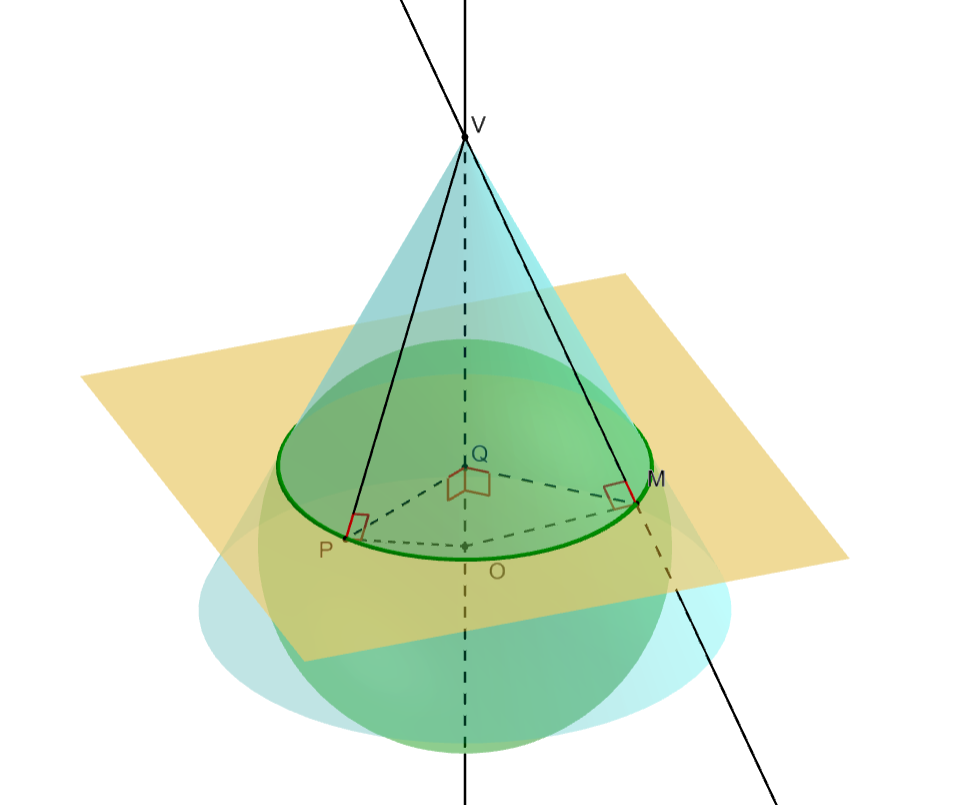
\includegraphics[width = 7cm]{./images/3d/lemme_cone_S.PNG}
\end{figure}
\end{minipage}
\hfill
\begin{minipage}{0.6\textwidth} % right side: text
    \vspace{0.5cm}
\begin{proof}
    \hspace{0.7\textwidth}

    Puisque les longueurs du triangle rectangle $\triangle VMO$ sont les mêmes pour tout point $M$, l'angle $\widehat{OVM} = \alpha$ est également constant.\\
Cela signifie que toutes les droites $VM$ forment un cône de révolution de sommet $V$, avec un angle d'ouverture $2\alpha$ avec la sphère $\mathcal{S}$ inscrite à l'intérieur.
Considérons l'axe du cône passant par $V$ et $O$. 
On peut former un autre triangle rectangle $\triangle VQM$, rectangle en $Q$.\\
La distance $\overline{VQ}$ 
est la même pour tout point $M$ de tangence puisque $\overline{VQ} = \overline{VM} \cos\alpha $.
Tous les points $M$ de tangence se trouvent dans un même plan perpendiculaire à l'axe $VO$. 
Par Pythagore, on a alors  $ \overline{QM}^2 =  \overline{VM}^2 - \overline{VQ}^2$ donc $ \overline{QM}$ est constante pour tout point de tangence $M$.

Le lieu des points de tangence $M$ est alors un cercle de centre $Q$.
\end{proof}
\end{minipage}

